\newpage
\begin{center}
    \textbf{\large 3. ДИФФУЗИЯ НА ЖИДКОСТНЫХ БИНОДАЛЯХ: ВЛИЯНИЕ ДАЛЬНОДЕЙСТВИЯ СИЛЫ ПРИТЯЖЕНИЯ}
\end{center}
\refstepcounter{chapter}
\addcontentsline{toc}{chapter}{3. ДИФФУЗИЯ НА ЖИДКОСТНЫХ БИНОДАЛЯХ: ВЛИЯНИЕ ДАЛЬНОДЕЙСТВИЯ СИЛЫ ПРИТЯЖЕНИЯ}


В данной главе используется моделирование молекулярной динамики для расчета фазовых диаграмм обобщенных систем Леннарда-Джонса с различными показателями притяжения.
Оценены коэффициенты диффузии и подвижности (обратной диффузии) и проанализированы спектры коллективного возбуждения на жидких бинодалиях. 
Отмечено, что зависимость коэффициента подвижности от температуры является линейной в широком диапазоне температур, а ее наклон увеличивается с увеличением показателя притяжения.
При отклонении подвижности от линейной зависимости дисперсионные соотношения коллективных возбуждений жидкости переходят от осцилирующего к монотонному виду.

\section{Роль диффузии в науке и технике}
\label{MACR-SecIntroduction}

Диффузия играет решающую роль в различных процессах переноса массы, начиная с науки и техники и заканчивая живой природой.
Диффузия выступает ключевым механизмом в биологических процессах~\cite{10.1016/j.bbagen.2013.09.037, 10.1038/s41598-018-22643-9}, а также в кинетике химических реакций.
Знание механизмов диффузии позволит добиться значительного прогресса в новых биотехнологиях и медицине, решить важные проблемы химической и фармакологической промышленности~\cite{10.1002/3527602836}.

Процесс диффузии очень хорошо изучен в газах и твердых телах.
Например, в кристаллических системах~\cite{10.1016/0079-6816(95)00039-2}, что связано с ее практической ценностью в металлургии для легирования~\cite{10.1016/s0924-0136(96)02826-9, 10.1016/j.actamat.2015.10.010, 10.1134/s1063783411110308} и эксплуатации полупроводниковой электроники~\cite{10.1103/physrevlett.84.4220, 10.1016/j.physrep.2009.10.003}.

В данной главе, используя метод молекулярной динамики (МД), моделируются обобщенные системы Леннарда-Джонса с различными показателями притяжения.
Рассчитаны температурные зависимости подвижности частиц (коэффициента обратной диффузии) на бинодали жидкость-газ. 
Здесь же рассмотрена связь между диффузией, дальнодействием межчастичного притяжения и свойствами коллективных возбуждений в простых жидкостях.

\section{Методы}
\label{MACR-SecMethods}

\subsection{Расчет фазовых диаграмм методами молекулярной динамики}
\label{MACR-SubSecMD}

В этой главе анализируются транспортные свойства и их связь с коллективными модами на жидких бинодальях.
Для систем, взаимодействующих через обобщенный потенциал Леннарда-Джонса (LJ$n$-$m$):
\begin{equation}
U_{n-m}(r)=4 \varepsilon\left[\left(\frac{\sigma}{r}\right)^{n}-\left(\frac{\sigma}{r}\right)^{m}\right]
\label{MACR-eq1}
\end{equation}
где $\epsilon$ и $\sigma$ -- характерные масштабы энергии и длины соответственно.
На протяжении всей статьи используются приведенные единицы измерения температуры $ T/ \epsilon \rightarrow T $, расстояния $ r/ \sigma \rightarrow r $ и плотности $ \rho \sigma ^ 3 \rightarrow n$.


Были рассмотрены потенциалы LJ$12$-$4$, LJ$12$-$5$, LJ$12$-$6$ и LJ$16$-$6$.
Чтобы сравнить полученные результаты для LJ$n$-$m$ с результатами для системы, в которой взаимодействия не являются сферически-симметричными, были также смоделировали этан~\cite{10.1021/acs.jced.6b01036}.
В выбранной модели молекула этана рассматривается как пара жестко связанных радикалов CH$_3$, взаимодействующих с радикалами других молекул через потенциал~\cite{10.1021/acs.jced.6b01036}:
\begin{equation}
U_{\rm {ethane}}(r) = \tilde \varepsilon\left[\left(\frac{\sigma}{r}\right)^{16}-\left(\frac{\sigma}{r}\right)^{6}\right],
\label{MACR-eq2}
\end{equation}
где $\tilde\varepsilon = 0,69396$ ккал/моль и $\sigma = 3,783$\AA.

Все МД-симуляции были выполнены в ансамбле NVT (N, V и T --количество частиц, объем системы и температура соответственно) с периодическими граничными условиями с использованием пакета моделирования \\  LAMMPS~\cite{10.1006/jcph.1995.1039}.
В первую очередь были рассчитаны линии бинодали~\cite{10.1021/jp806127j, 10.1021/jp1117213}.
Исходное состояние системы формировалось в два этапа: (i) кубическая область моделирования заполнялась равновесным кристаллом (в нашем случае ГЦК) из $N$ частиц с плотностью, соответствующей близкому к нулю давлению; 
(ii) область моделирования была расширена в направлении осей $x$ так, чтобы окончательная средняя плотность системы $\rho_a$ стала равной значениям, указанным в таблице~\ref{MACR-Table1}.
Результирующее начальное состояние показано на рис.~\ref{MACR-Figure1}(а). 
Затем температура системы линейно увеличивалась от $T_{start}$ до $T_{stop}$ в течение $n_{step}$ шагов моделирования с временным шагом $\Delta t$.
Конденсированная фаза в какой-то момент начинает испаряться, образуя сосуществование газа и конденсата, если температура ниже критической, как показано на рис.~\ref{MACR-Figure1}(b).
Принципиально то, что полученное таким образом состояние системы почти всегда имеет границы фаз, ортогональные оси $x$.
В результате плотности $\rho_g$ и $\rho_c$ газовой и конденсированной фаз соответственно могут быть рассчитаны путем подгонки профиля плотности $\rho(x)$ выражением~\cite{10.1021/jp806127j, 10.1021/jp1117213}:

\begin{equation}
    \rho(x)=\frac{\rho_{l}+\rho_{g}}{2}-\frac{\rho_{l}-\rho_{g}}{2} \tanh \left(\frac{|x|-L}{\delta}\right),
    \label{MACR-eq3}
\end{equation}
где $L$ — половина длины области моделирования, занимаемой жидкой фазой, а $\delta$ — характерная ширина границы раздела.
Пример профиля плотности системы и его аппроксимация уравнением~\eqref{MACR-eq3} показаны на рис.~\ref{MACR-Figure1}(c) гистограммой и красной линией соответственно.
Параметры моделирования для рассмотренных моделей сведены в табл.~\ref{MACR-Table1}.

\begin{table}[]
\centering
\begin{tabular}{|lllllcl|}
\hline
\multicolumn{1}{|l|}{Potential} & \multicolumn{1}{l|}{$\rho_a$} & \multicolumn{1}{l|}{$r_c$} & \multicolumn{1}{l|}{$T_{start}$} & \multicolumn{1}{l|}{$T_{stop}$} & \multicolumn{1}{l|}{$n_{step}$}                       & $\Delta t$                          \\ \hline
\multicolumn{7}{|c|}{Значения в безразмерных единицах:}                                                                                                                                                                                                         \\ \hline
\multicolumn{1}{|l|}{LJ12-4}    & \multicolumn{1}{l|}{0.25}     & \multicolumn{1}{l|}{15.0}  & \multicolumn{1}{l|}{1.0}         & \multicolumn{1}{l|}{5.5}        & \multicolumn{1}{c|}{\multirow{4}{*}{$3 \times 10^6$}} & \multirow{4}{*}{$5 \times 10^{-4}$} \\ \cline{1-5}
\multicolumn{1}{|l|}{LJ12-5}    & \multicolumn{1}{l|}{0.25}     & \multicolumn{1}{l|}{10.0}  & \multicolumn{1}{l|}{0.8}         & \multicolumn{1}{l|}{2.4}        & \multicolumn{1}{c|}{}                                 &                                     \\ \cline{1-5}
\multicolumn{1}{|l|}{LJ12-6}    & \multicolumn{1}{l|}{0.35}     & \multicolumn{1}{l|}{8.0}   & \multicolumn{1}{l|}{0.5}         & \multicolumn{1}{l|}{1.4}        & \multicolumn{1}{c|}{}                                 &                                     \\ \cline{1-5}
\multicolumn{1}{|l|}{LJ16-6}    & \multicolumn{1}{l|}{0.31}     & \multicolumn{1}{l|}{8.0}   & \multicolumn{1}{l|}{0.8}         & \multicolumn{1}{l|}{1.6}        & \multicolumn{1}{c|}{}                                 &                                     \\ \hline
\multicolumn{7}{|c|}{Единицы измерения СИ:}                                                                                                                                                                                                                     \\ \hline
\multicolumn{1}{|l|}{Ethane}    & \multicolumn{1}{l|}{$0.22\mathrm{\frac{g}{cm^3}}$}     & \multicolumn{1}{l|}{$25\text{\AA}$}    & \multicolumn{1}{l|}{$80\,\mathrm{K}$}          & \multicolumn{1}{l|}{$320\,\mathrm{K}$}        & \multicolumn{1}{l|}{$2 \times 10^6$}                  & $2\,\mathrm{\text{фс}}$                                   \\ \hline
\end{tabular}
\caption{Параметры, используемые в МД-моделировании для бимодальных расчетов: где $\rho$ — средняя плотность системы, $r_c$ — радиус отсечки, $T_{start}$ и $T_{stop}$ — начальная и конечная температуры моделирования, соответственно, $n_{step}$ — количество шагов моделирования, а $\Delta t$ — временной шаг.}
\label{MACR-Table1}
\end{table}


\begin{figure}[!t]
\centering
    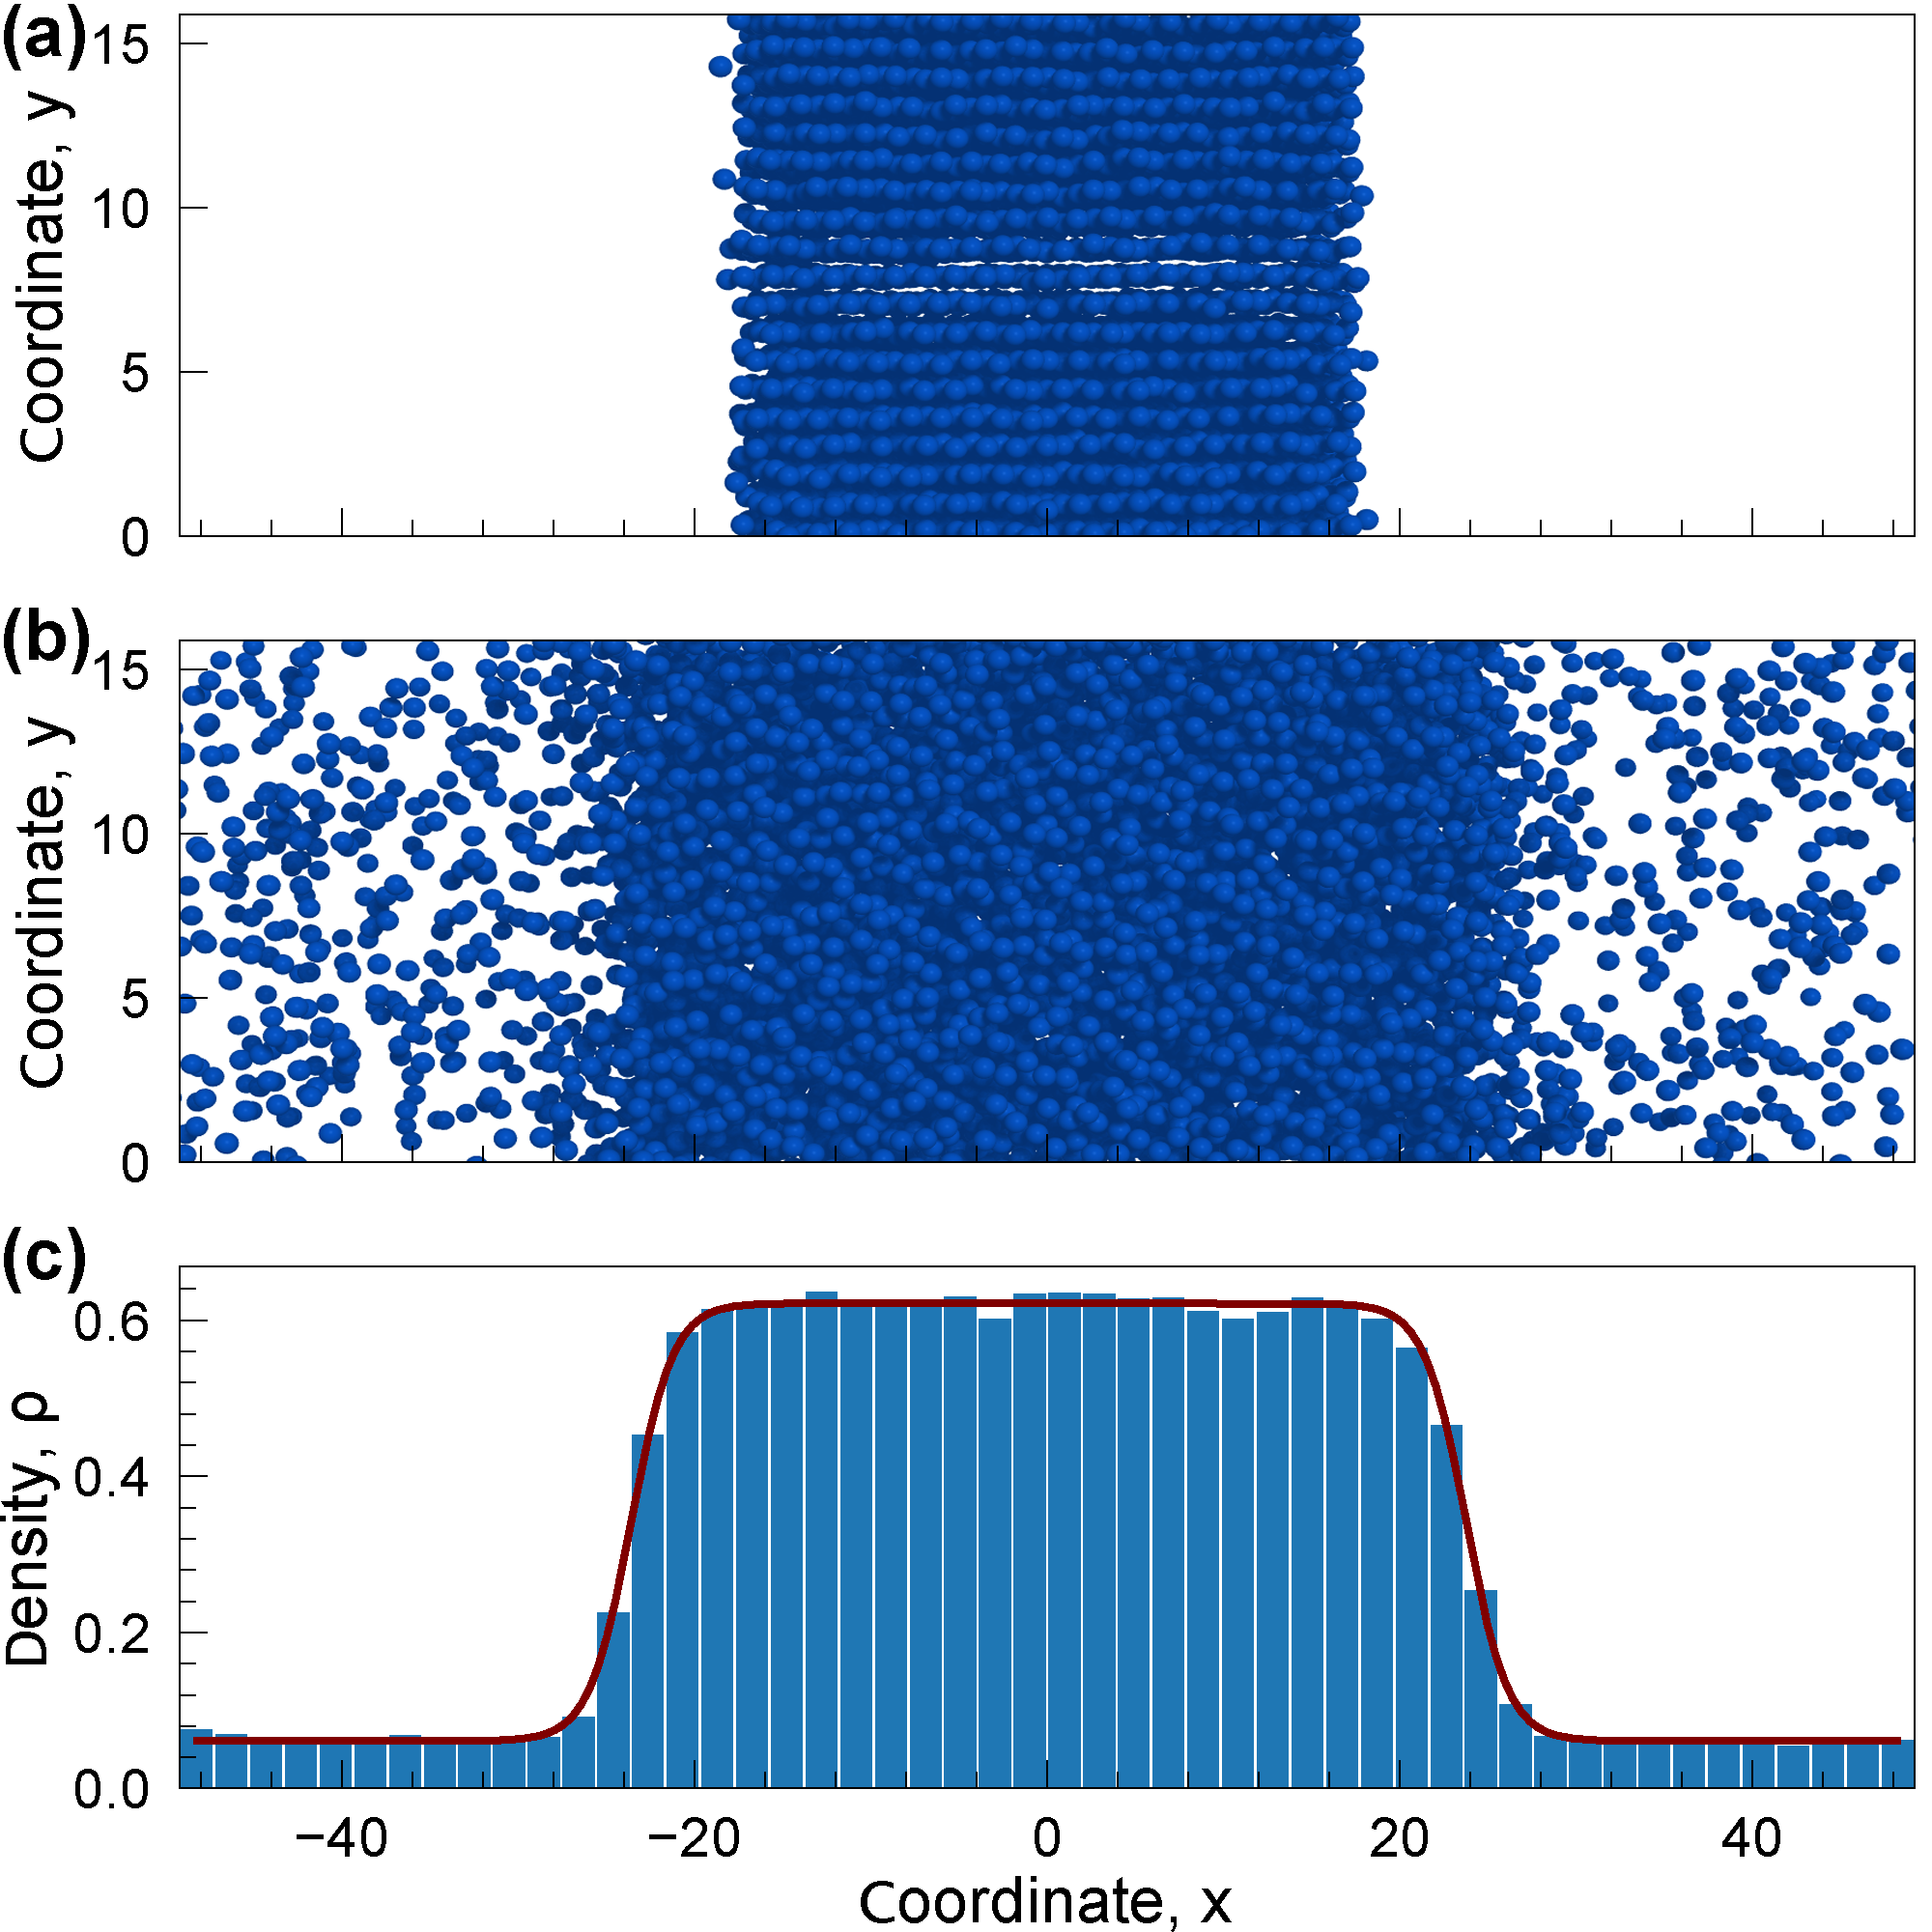
\includegraphics[width=150mm]{MACR-Figure1.png}
    \caption{(a) Система частиц для расчета фазовой диаграммы.
    Система частиц с потенциалом взаимодействия LJ12-6 при температуре $T=1.13$ в виде плоского слоя.
    (b) Профиль плотности системы вдоль оси $x$.
    Область с высокой плотностью представляет собой конденсат, с низкой -- газ.
    Темно-красная линия представляет собой аппроксимацию профиля плотности уравнением~\eqref{MACR-eq3}.}
\label{MACR-Figure1}
\end{figure}


\begin{figure}[!t]
\centering
    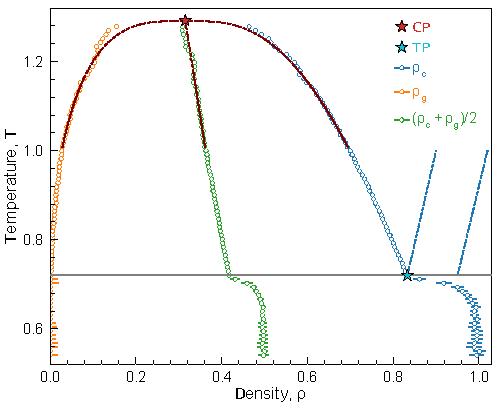
\includegraphics[width=150mm]{MACR-Figure2.pdf}
    \caption{Фазовая диаграмма системы LJ12-6.
    Оранжевым и синим цветами обозначены символы плотности газа и конденсата соответственно, полученные путем подгонки данных МД по уравнению~\eqref{MACR-eq3}.
    Зеленые символы -- медиана $\rho_m=(\rho_g+\rho_c)/2$.
    Сплошная красная линия соответствует уравнению~\eqref{MACR-eq4}.
    Тройные и критические точки -- синие и красные звездочки соответственно.
    }
\label{MACR-Figure2}
\end{figure}

Вблизи критической температуры расчет плотности газа и жидкости становится затруднительным из-за усиленных флуктуаций плотности.
Однако положение критической точки на фазовой диаграмме можно вычислить, аппроксимируя жидкостную и газообразную бинодальные ветви вблизи критической точки выражением~\ref{MACR-eq4}.

В трехмерии критический индекс $\beta_c = 0,5$ для потенциала LJ$12-4$, тогда как $\beta_c = 0,325$ для LJ$12$-$5$, LJ$12$-$6$, LJ$16$-$6$ и этана, согласно предыдущим результатам~\cite{10.1021/acs.jced.6b01036,10.1021/jp9072137,10.1103/physrevlett.89.025703}.

Пример полученных бинодалей для LJ12-6 и их аппроксимации уравнением~\eqref{MACR-eq4} показаны на рис.~\ref{MACR-Figure2}.
Обратите внимание, что на конденсированной бинодали имеется явный излом (см. рис.~\ref{MACR-Figure2}), который указывает на падение плотности при плавлении и соответствует положению тройной точки.
Полученные значения $A$ и $a$ из уравнения~\eqref{MACR-eq4}, а также значения плотности и температуры критических и тройных точек для рассматриваемых систем представлены в таблице~\ref{MACR-Table2}.

\begin{figure}[!t]
\centering
    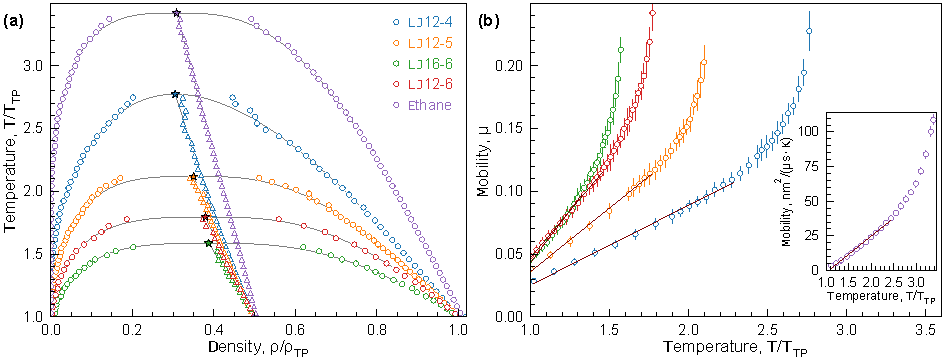
\includegraphics[width=\linewidth]{MACR-Figure3.pdf}
    \caption{(а) Фазовые диаграммы рассматриваемых систем. 
    Фазовые диаграммы рассчитывались методом двухфазного моделирования, который описан в разделе~\ref{MACR-SecMethods}.
    Цветные точки обозначают рассчитанные бинодали, треугольники -- срединные точки.
    Сплошные серые кривые показывают диапазон температур, используемый для аппроксимации и определения параметров в уравнении ~\eqref{MACR-eq4}.
    Штриховые серые кривые соответствуют экстраполированным биноидам.
    (б) Температурная зависимость подвижности частиц.
    Подвижность частиц была рассчитана на жидких бинодальях с использованием метода, описанного в разделе~\ref{MACR-SecMethods}.
    Точки, соответствующие экстраполированным бинодалим, отмечены серым цветом. 
    Прямые линии -- линейная аппроксимация подвижности.
    На вставке показана расчетная подвижность метана.}
\label{MACR-Figure3}
\end{figure}

\subsection{Расчет диффузии и спектров на бинодали}

Далее для расчета подвижности на конденсированной бинодали моделировались системы с плотностью и температурой, взятыми из полученных фазовых диаграмм.
Обобщенные систем Леннарда-Джонса с $N = 4,0 \times 10 ^ 3$ моделировались с шагом по времени $1,5 \times 10 ^ 5$.
Для этана использовались $N = 1,065 \times 10 ^ 4 $ молекул и проведены моделирования с шагом по времени $7.0 \times 10^5 $.
Для релаксации системы использовались первые $ 5.0 \times 10 ^ 4 $ временных шагов для обобщенных LJ-систем и $ 5.0 \times 10 ^ 5 $ для этана.
Остальные параметры были такими же, как и при расчете фазовых диаграмм.

Коэффициент самодиффузии $D$ определялся по среднеквадратичному отклонению частиц:
\begin{equation}
    \sigma^2(t) = \sum\limits_{\alpha = 1}^{N} (r_{\alpha}(t) - r_{\alpha}(0))^2 / N, \quad \sigma^2(t) = 6Dt,
    \label{MACR-eq5}
\end{equation}
где $\sigma$ — среднеквадратичное отклонение, а $t$ — время.
Подвижность $\mu$ связана с коэффициентом диффузии соотношением Эйнштейна
\begin{equation}
    \mu = \frac{D}{T},
    \label{MACR-eq6}
\end{equation}
где $T$ — температура системы.

Наконец, спектры возбуждения были получены с использованием обработки тока скорости~\cite{10.1063/1.5050708}:
\begin{equation}
    C_{L, T}(\mathbf{q}, \omega)=\int dt e^{i \omega t} \text{Re} \left\langle\mathbf{j}_{L, T}(\mathbf{q}, t) \mathbf{j}_{L, T}(-\mathbf{q}, 0)\right\rangle,
    \label{MACR-eq7}
\end{equation}
где ${\bf k}$ и $\omega$ — волновой вектор и частота,
$\mathbf{j}_{L}=\mathbf{q}(\mathbf{j} \cdot \mathbf{q} ) / q^{2}$ и $\mathbf{j}_{T}=(\mathbf{j \cdot e_{\perp})e_{\perp}}$ — продольная ($L$) и поперечная ($T$) компоненты тока частиц,\\
$\mathbf{j}(\mathbf{q}, t)=N^{-1} \sum_{s} \mathbf{v}_{s}(t) \ exp \left(i \mathbf{q} \mathbf{r}_{s}(t)\right)$ и $\mathbf{v}_{s}(t)=\dot{\mathbf{r} }_{s}(t)$ — скорость $s$-й частицы.
Суммирование ведется по всем $N$ частицам в системе.
Усреднение по каноническому ансамблю обозначается $\langle\cdots\rangle$. 
Анализ $C_{L, T}(\mathbf{q}, \omega)$ проводился с помощью методов из работы~\cite{10.1038/s41598-019-46979-y}, что позволило получить дисперсионные соотношения продольной и поперечной мод.

МД-моделирование для расчета спектров возбуждения отличается от моделирования для подвижности только длительностью временного шага. Для LJ$12$-$4$ и LJ$16$-$6$ шаг по времени был выбран как $\Delta t = 1 \times 10 ^ {-4} \sqrt {m \sigma ^ 2 / \epsilon}$, а для LJ$12$-$5$ и LJ$12$-$6$ -- $\Delta t = 5 \times 10 ^ {-4} \sqrt {m \sigma ^ 2 / \epsilon}$.

\begin{figure}[!t]
\centering
    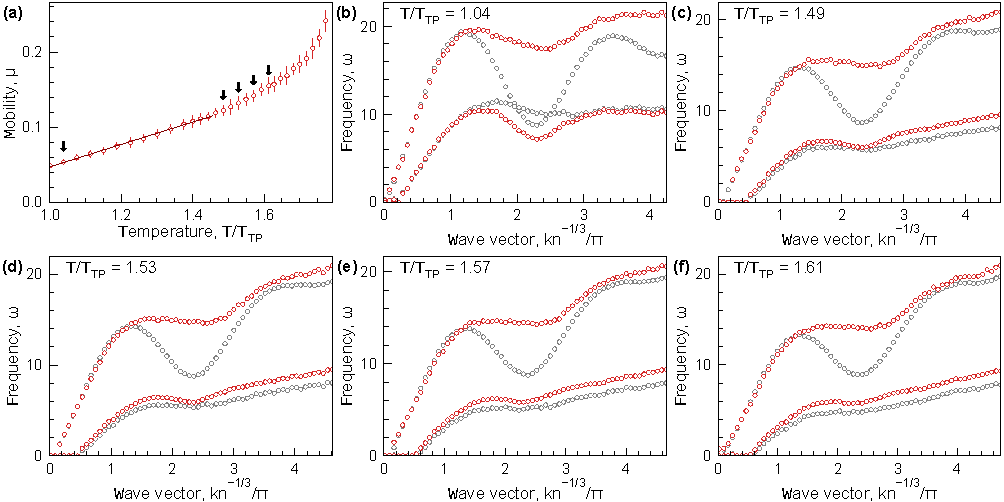
\includegraphics[width=160mm]{MACR-Figure4.pdf}
    \caption{(a) Температурная зависимость подвижности системы LJ$12$-$6$ вдоль жидкостной бинодали.
    Температуры, при которых рассчитывались спектры возбуждения, указаны черными стрелками.
    (b) - (f) спектры возбуждения LJ$12$-$6$ систем.
Спектры рассчитывались путем анализа скорости течения (уравнение~\eqref{MACR-eq7}) так же, как в Ref.~\cite{10.1038/s41598-019-46979-y}.
    Красный цвет соответствует гибридным модам, серый — результатам анализа отдельных мод~\cite{10.1038/s41598-019-46979-y}.
    В левом верхнем углу указаны пониженные температуры.}
\label{MACR-Figure4}
\end{figure}

\section{Результаты}
\label{MACR-SecResults}

Результаты расчета границ сосуществования газа и жидкости показаны на рис.~\ref{MACR-Figure3}(а).
Цветные точки обозначают бинодали, треугольники -- срединные точки.
Точки, которые использовались для аппроксимации [с использованием уравнения~(\ref{MACR-eq4})], выделены сплошной серой линией.
Экстраполированные бинодали обозначены пунктирной серой линией.
Для каждой рассматриваемой системы температура и плотность выражаются в единицах температуры и плотности тройной точки соответственно.
Последние значения вместе с параметрами критических точек приведены в Таб.~\ref{MACR-Table2}.

\begin{table}[h!]
    \centering{
    \begin{tabular}{C{1.5cm}|C{1.0cm}|C{1.0cm}|C{1.0cm}|C{1.0cm}|C{1.0cm}|C{1.0cm}}
        LJn-m & $T_{\rm CP}$ & $\rho_{\rm CP}$ & $T_{\rm TP}$ & $\rho_{\rm TP}$ & $A$ & $a$ \\ \hline
        LJ12-4 & 4.85 & 0.291 & 1.75 & 0.952 & 0.559 & 0.107 \\
        LJ12-5 & 2.18 & 0.304 & 1.03 & 0.867 & 0.804 & 0.208 \\
        LJ12-6 & 1.29 & 0.315 & 0.72 & 0.830 & 1.002 & 0.326 \\
        LJ16-6 & 1.55 & 0.316 & 0.98 & 0.816 & 0.969 & 0.334 \\
        Ethane & 305.3 & 206.7 & 90.34 & 651.9 & 113.1 & 1.158
    \end{tabular}

    }
    \caption{Значения плотностей и температур критических и тройных точек и параметры аппроксимации по уравнению~\eqref{MACR-eq4} для рассматриваемых моделей.
    Для обобщенных систем LJ температуры и плотности даны в сокращенных единицах.
    Для этана температура выражена в К, а плотность выражена в $\text{кг}/\text{м}^3$.
    Параметры критической и тройной точек для этана взяты из работы~\cite{10.1063/1.555785}.}
    \label{MACR-Table2}
\end{table}

\begin{figure}[!t]
\centering
    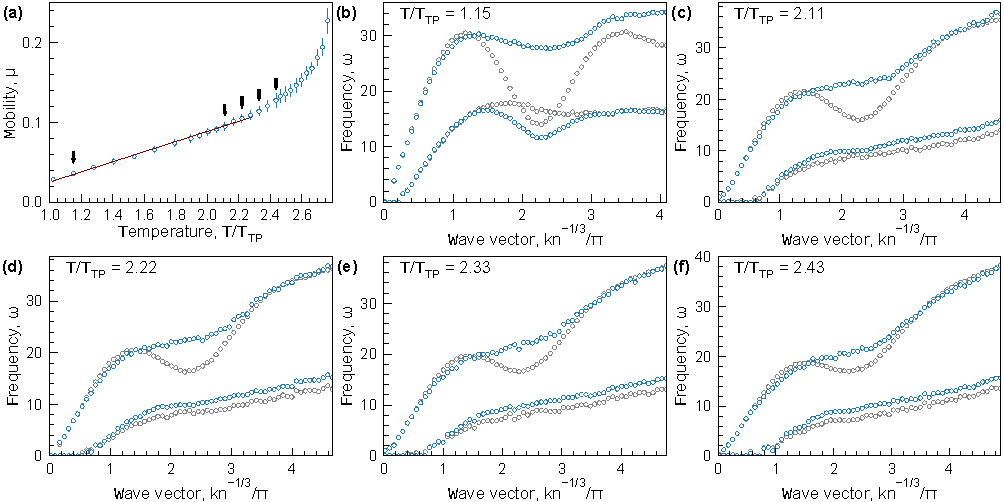
\includegraphics[width=160mm]{MACR-Figure5.pdf}
    \caption{Результаты для потенциала LJ$12$-$4$.
    Рисунок аналогичен рисунку~\ref{MACR-Figure4}(a)-(f).}
\label{MACR-Figure5}
\end{figure}


Замечено, что с увеличением дальнодействия потенциала увеличиваются как температуры тройных и критических точек, так и их отношение $T_{\rm CP}/T_{\rm TP}$.

Затем по рассчитанным фазовым диаграммам была вычислена подвижность частиц при плотностях и температурах, соответствующих бинодали жидкости.
Полученная зависимость подвижности частиц от температуры представлена на рис.~\ref{MACR-Figure3}(b).
Цветные точки на (b) соответствуют цветным точкам на (a).
Серые точки обозначают подвижности на экстраполированных частях бинодали.

\begin{figure}[!t]
\centering
    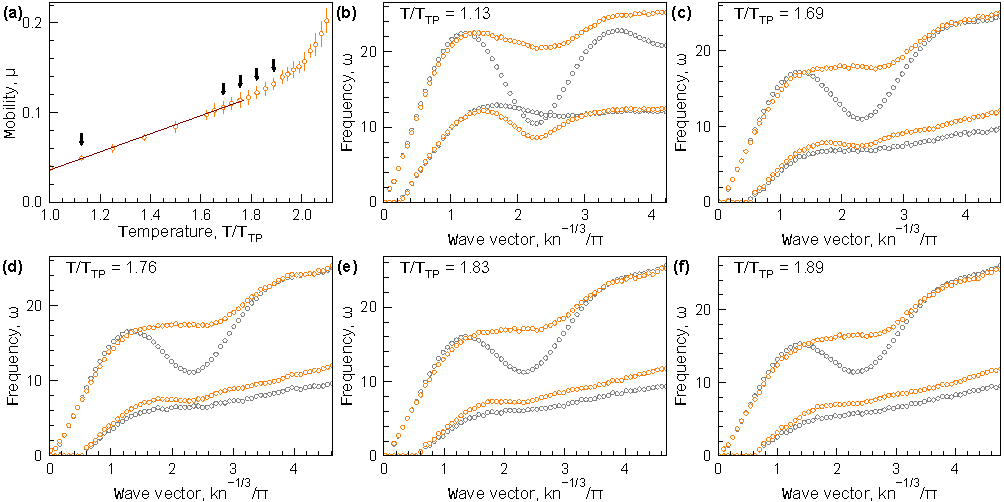
\includegraphics[width=160mm]{MACR-Figure6.pdf}
    \caption{Результаты для потенциала LJ$12$-$5$.
    Рисунок аналогичен рисунку~\ref{MACR-Figure4}(a)-(f).}
\label{MACR-Figure6}
\end{figure}

Отметим, что при низких температурах подвижность на бинодали имеет линейную зависимость от температуры.
Ее наклон увеличивается с уменьшением дальнодействующего характера потенциала взаимодействия (т.е. с увеличением показателя притяжения).
Линейная зависимость сохраняется до определенной температуры, после которой происходит отклонение от линейной зависимости.
Возникновение такой нелинейности может быть связано с особенностями коллективной динамики частиц, которые должны коррелировать со спектрами коллективных возбуждений.

Вычисленные спектры системы LJ$12$-$6$ показаны на рис.~\ref{MACR-Figure4}.
На рисунке~\ref{MACR-Figure4}(а) изображены зависимости подвижности от температуры, а черными стрелками указаны температуры, при которых рассчитывались спектры. 
Были выбраны точки вблизи температуры, при которой наблюдается начало нелинейной зависимости, а также температура вблизи тройной точки.
На рисунке~\ref{MACR-Figure4}(b)-(f) показаны вычисленные дисперсии продольных и поперечных мод в этих точках.
Красный цвет соответствует модели с двумя осцилляторами, а серый — одномодовому анализу~\cite{10.1038/s41598-019-46979-y}.

Нетрудно заметить, что по мере приближения температуры к точке, соответствующей возникновению нелинейной зависимости, дисперсионные соотношения демонстрируют переход от осциллирующей к монотонной зависимости от волнового числа.
Таким образом, качественное изменение температурной зависимости подвижности частиц сопровождается изменением спектров возбуждения.
Наблюдаемая картина не является особенной для системы LJ$12$-$6$.
Аналогичная тенденция замечена и в других исследованных обобщенных ЛД-систем.
Это наблюдение дает новое свидетельство тесной связи между диффузией и свойствами коллективных возбуждений.


\begin{figure}[!t]
\centering
    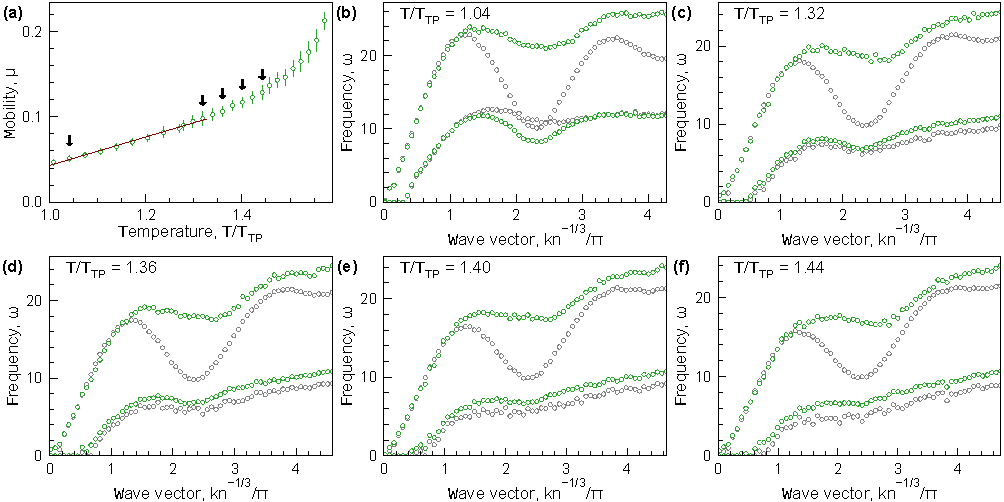
\includegraphics[width=160mm]{MACR-Figure7.pdf}
    \caption{Результаты для потенциала LJ$16$-$6$.
    Рисунок аналогичен рисунку~\ref{MACR-Figure4}(a)-(f).}
\label{MACR-Figure7}
\end{figure}


\section{Заключение главы}
\label{MACR-SecConclusions}

В данной главе исследовано влияние формы потенциала парного взаимодействия на фазовые диаграммы и подвижность частиц в жидкой фазе.
Были рассчитаны кривые сосуществования газа и жидкости для потенциалов с переменным дальнодействием притяжения.
Отмечено, что с увеличением дальнодействующего характера потенциала температуры тройной и критической точек, а также их отношение $T_{\rm CP}/T_{\rm TP}$ увеличиваются.
Коэффициент диффузии и обратный ему коэффициент подвижности вычислялись на жидких бинодалиях.
Было обнаружено, что температурная зависимость подвижности линейна в широком диапазоне температур с тем большим наклоном, чем меньше диапазон притяжения.
Кроме того, установлено, что начало нелинейной температурной зависимости подвижности при высоких температурах совпадает с переходом дисперсионных зависимостей коллективных возбуждений от осциллирующей к монотонной зависимости от волнового числа.
Полученные результаты дают возможность для дальнейшего изучения диффузии и ее связи с коллективными процессами в конденсированных многочастичных системах.
